\chapter{Results}\label{chap:results}

\section{Controller Requirements}
\begin{itemize}
    \item It should be possible to select the area in which the bathymetric measurements are to be performed.
    \item The ASV should be able to autonomously plan and follow a route, such that the entire survey area is mapped.
    \item The controller should be robust to external disturbances.
    \item THU should not exceed 30cm with a 95\% confidence interval.
\end{itemize}

The are to survey can be selected by giving the four coordinates of the corners and the algorithm will select the needed waypoints to cover it, depending on the beamwidth.

Once this waypoints are selected the outer controller set the appropriate references for speed and heading to the inner controller. The performance of the outer controller when using both inner controllers can be seen in \autoref{sec:pathSim}. The figures are included here as well, but in this case to check the fulfillment of the requirements.

\autoref{fig:path_lqr} shows the simulation results of the path followed by the vessel in the survey area when using the LQR as inner controllerr. The results are also shown in \autoref{fig:distlqr2} by plotting the error to the reference path.
\begin{figure}[H]
    \captionbox  
    {            
        Performance of the path following algorithm based on $\psi_\mathrm{ref}=\chi-\beta$ and using the LQR inner controller. The system is experiencing wind and wave disturbances, model perturbations and measurement noise.            
        \label{fig:path_lqr}                               
    }                                                                
    {                                                                 
        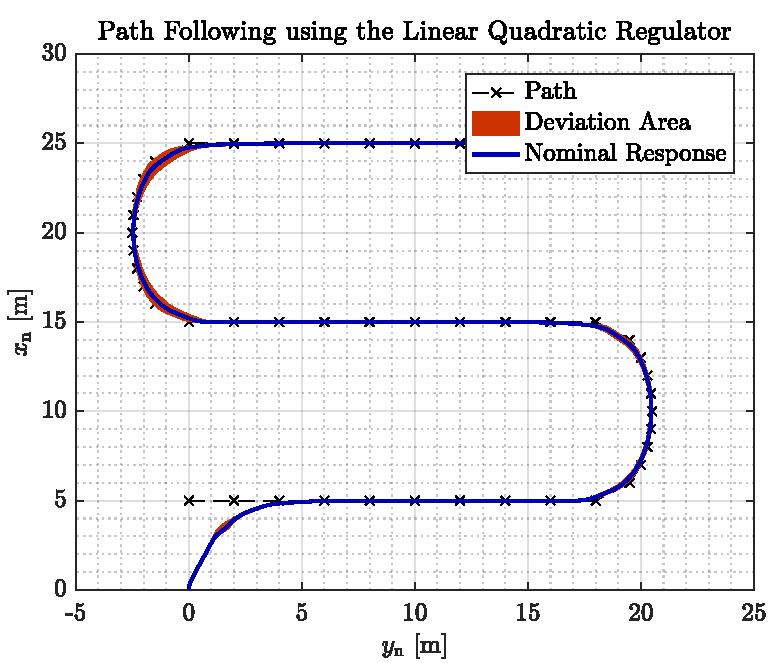
\includegraphics[width=.45\textwidth]{figures/path_lqr}    
    }                                                                  
    \hspace{5pt}                                                        
    \captionbox 
    {       
        Distance to the path when using the algorithm based on $\psi_\mathrm{ref}=\chi-\beta$ and the LQR inner controller.                                                                  %\                         %\
        \label{fig:distlqr2}                                  
    }                                                                          
    {                                                                            
        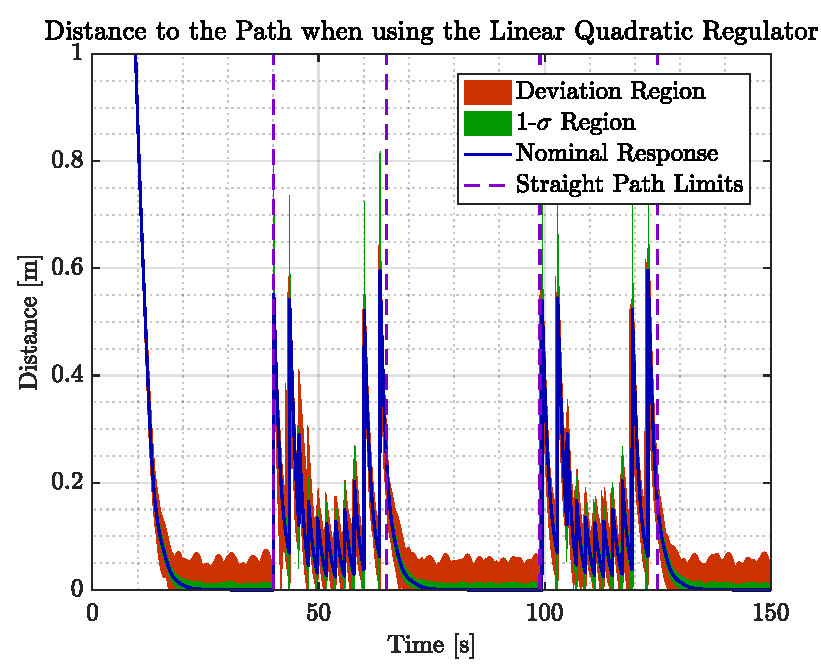
\includegraphics[width=.45\textwidth]{figures/dist_lqr}          
    }                                                                            
\end{figure}
It can be seen that the distance to the path is kept below 10 cm in the straight parts of the path, which correspond to the given area, while the distance on the curved section does not matter for the survey task. Since the system has a requirement of 30 cm, this is sufficiently fulfilled in simulation with the Linear Quadratic Regulator.

The path has also been tracked using the $\mathcal{H}_\infty$ inner controller as seen below.
\begin{figure}[H]
    \captionbox 
    {   
        Performance of the path following algorithm based on $\psi_\mathrm{ref}=\chi-\beta$ and using the $\mathcal{H}_\infty$ inner controller. The system is experiencing wind and wave disturbances, model perturbations and measurement noise. \label{fig:path_rob2}
    }                                                                 
    {                                                                  
        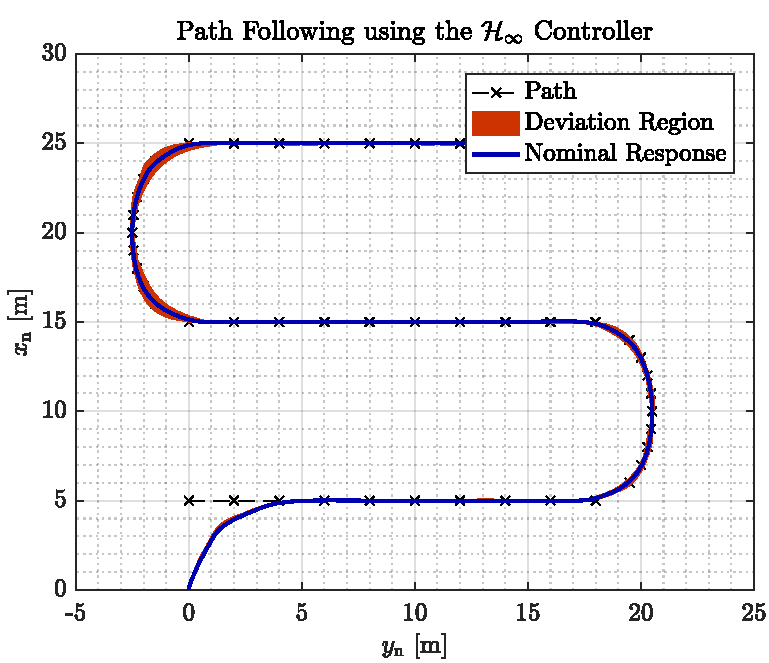
\includegraphics[width=.45\textwidth]{figures/path_rob}         
    }                                                                    
    \hspace{5pt}                                                          
    \captionbox  
    {      
        Distance to the path when using the algorithm based on $\psi_\mathrm{ref}=\chi-\beta$ and the $\mathcal{H}_\infty$ inner controller. \label{fig:dist_rob2}
    }                                                                          
    {
        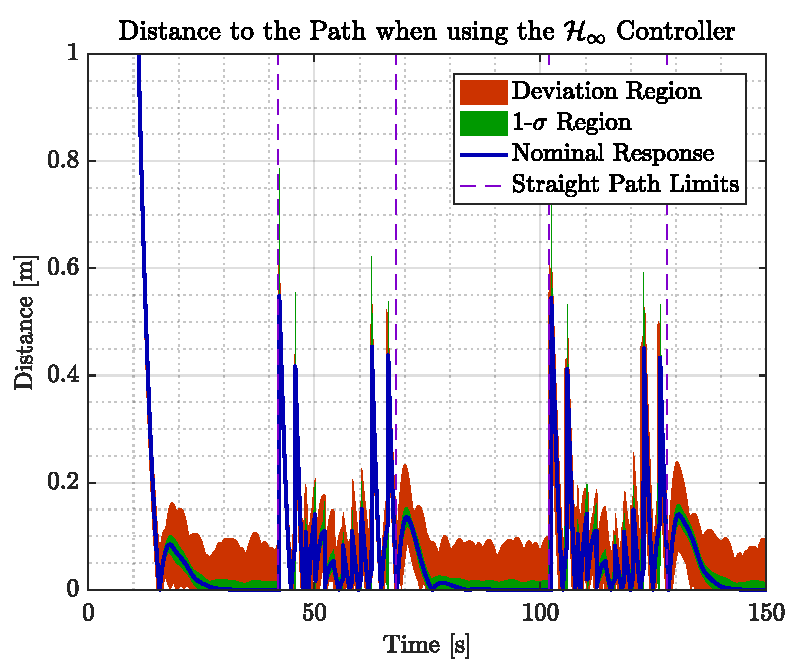
\includegraphics[width=.45\textwidth]{figures/dist_rob}
    }
\end{figure}
In this case the requirement in the straight part of the path is also fulfilled since the distance stays always below 15 cm.

According to the results of the simulations, it can be said that the vessel follows the path through the waypoints when they are part of a straight line section of the path. In curved sections, the vessel joins smoothly the straight line segments that approximate the curve. 

Since the simulation includes as well disturbances, noise and parameter variation, the robustness of the controller against them has also been tested. In many cases, and especially for bathymetric measurements, the algorithm can be considered suitable.


\section{Implementation Requirements}
\begin{itemize}
    \item The ASV should record and store data locally for extraction at the end of the survey.
    \item It should be possible to give the ASV a command to stop and steer it back to land.
\end{itemize}

We rosbag the files to save all the topics
Keyboard teleop node and VPN connection to run the nodes and stop them